
\begin{figure}[tb]
{\tt \small
\hrule
\vspace{0.2cm}
\begin{lstlisting}[mathescape]
$\mathbf{let}$ $\mathbf{rec}$ unifyReal $\mathtt{s_1}$ $\mathtt{u_1}$ $\mathtt{p_1}$ $\mathtt{s_2}$ $\mathtt{u_2}$ $\mathtt{p_2}$ = $\mathbf{match}$ (!$\mathtt{s_1}$,!$\mathtt{u_1}$,!$\mathtt{p_1}$) $\mathbf{with}$
  ($\mathbf{in}$t($\mathtt{s_1}'$),$\mathbf{in}$t($\mathtt{u_1}'$),$\mathbf{in}$t($\mathtt{p_1}'$)) $\rightarrow$  
    ($\mathbf{match}$ (!$\mathtt{s_2}$,!$\mathtt{u_2}$,!$\mathtt{p_2}$) $\mathbf{with}$
       ($\mathbf{in}$t($\mathtt{s_2}'$),$\mathbf{in}$t($\mathtt{u_2}'$),$\mathbf{in}$t($\mathtt{p_2}'$)) $\rightarrow$ 
         $\mathbf{let}$ s = $\mathbf{if}$ ($\mathtt{s_1}'$=$\mathtt{s_2}'$) $\mathbf{then}$ $\mathtt{s_1}'$ $\mathbf{else}$ 2 $\mathbf{in}$
         $\mathbf{let}$ u = max $\mathtt{u_1}'$ $\mathtt{u_2}'$ $\mathbf{in}$
         $\mathbf{let}$ p = $\mathbf{if}$ ($\mathtt{u_1}'$>=$\mathtt{u_2}'$) $\mathbf{then}$ m$\mathbf{in}$ $\mathtt{p_1}'$ ($\mathtt{u_1}'$ - $\mathtt{u_2}'$ + $\mathtt{p_2}'$) 
                $\mathbf{else}$ m$\mathbf{in}$ $\mathtt{p_2}'$ ($\mathtt{u_2}'$ - $\mathtt{u_1}'$ + $\mathtt{p_1}'$) 
         $\mathbf{in}$ $\mathbf{if}$ (p>0) $\mathbf{then}$ 
              ($\mathtt{s_1}$ := $\mathbf{in}$t(s) ; $\mathtt{s_2}$ := $\mathbf{in}$t(s) ; $\mathtt{u_1}$ := $\mathbf{in}$t(u) ; 
               $\mathtt{u_2}$ := $\mathbf{in}$t(u) ; $\mathtt{p_1}$ := $\mathbf{in}$t(p) ; $\mathtt{p_2}$ := $\mathbf{in}$t(p))
           $\mathbf{else}$ $\mathbf{raise}$ (Error ("Type "^(printExpr (TFloat($\mathtt{s_1}$,$\mathtt{u_1}$,$\mathtt{p_1}$)))^" is 
           not compatible $\mathbf{with}$ type "^(printExpr (TFloat($\mathtt{s_2}$,$\mathtt{u_2}$,$\mathtt{p_2}$))) ) )
     | (TypeVar(refS,strS),TypeVar(refU,strU),TypeVar(refP,strP)) $\rightarrow$ 
          refS := Some(!$\mathtt{s_1}$) ; refU := Some(!$\mathtt{u_1}$) ; refP := Some(!$\mathtt{p_1}$) 
     | _ $\rightarrow$ solveLT !$\mathtt{s_1}$ !$\mathtt{s_2}$ !$\mathtt{u_1}$ !$\mathtt{u_2}$ !$\mathtt{p_1}$ !$\mathtt{p_2}$ 
    )
| (TypeVar(refS,strS),TypeVar(refU,strU),TypeVar(refP,strP)) $\rightarrow$ 
    (($\mathbf{match}$ !refS $\mathbf{with}$
        None $\rightarrow$ refS := Some(!$\mathtt{s_2}$) 
      | Some($\mathtt{s_1}$) $\rightarrow$ unify $\mathtt{s_1}$ !$\mathtt{s_2}$) ;
     ($\mathbf{match}$ !refU $\mathbf{with}$
        None $\rightarrow$ refU := Some(!$\mathtt{u_2}$) 
      | Some($\mathtt{u_1}$) $\rightarrow$ unify $\mathtt{u_1}$ !$\mathtt{u_2}$) ; 
     ($\mathbf{match}$ !refP $\mathbf{with}$
        None $\rightarrow$ refP := Some(!$\mathtt{p_2}$) 
      | Some($\mathtt{p_1}$) $\rightarrow$ unify $\mathtt{p_1}$ !$\mathtt{p_2}$) 
    ) 
| _ $\rightarrow$ ($\mathbf{match}$ (!$\mathtt{s_2}$,!$\mathtt{u_2}$,!$\mathtt{p_2}$) $\mathbf{with}$
          (TypeVar(refS,strS),TypeVar(refU,strU),TypeVar(refP,strP)) $\rightarrow$
             $similar\ to\ previous\ case$ 
        | _ $\rightarrow$ $\mathbf{if}$ (($\mathtt{s_1}$=$\mathtt{s_2}$) && ($\mathtt{u_1}$=$\mathtt{u_2}$) && ($\mathtt{p_1}$=$\mathtt{p_2}$)) $\mathbf{then}$ () 
               $\mathbf{else}$ solve !$\mathtt{s_1}$ !$\mathtt{s_2}$ !$\mathtt{u_1}$ !$\mathtt{u_2}$ !$\mathtt{p_1}$ !$\mathtt{p_2}$
       )
\end{lstlisting}
}
\vspace{0.2cm}
\hrule
\caption{\label{unireal}Unification procedure for types \texttt{real}.}
\end{figure}

\section{Type System Implementation}
\label{implem}

In this section, we give some details about the implementation of our type system
in \texttt{Numl}. Section \ref{unif} deals with  the unification algorithm and Section
\ref{morex} presents examples of typable programs in complement to  the 
introductory examples of Section \ref{over}.

\subsection{Unification Algorithm}
\label{unif}

In this section, we describe how the type system introduced in Section \ref{infe} is implemented.
%More precisely, we show how the type inference and unification algorithms work.
Basically, we use a unification-based type inference in which type variables are represented by
reference cells. The type \texttt{real} also stores the format $\{s,u,p\}$ into reference cells,
so that it can be modified when unifying two terms of type \texttt{real}. 

The type inference and unification algorithms are classical excepted for the unification of two
  \texttt{real} types, done by the function \texttt{unifyReal} displayed in Figure \ref{unireal}
and which requires, in certain cases, a call to a SMT solver (in practice we use \texttt{Z3} \cite{Mou08}).
The function \texttt{unifyReal} takes as arguments the formats $\phi_1=\{s_1,u_1,p_1\}$ and 
$\phi_2=\{s_2,u_2,p_2\}$ of the types to be unified.


\begin{figure}[tb]
  \begin{center}
\hrule
\vspace{0.1cm}
    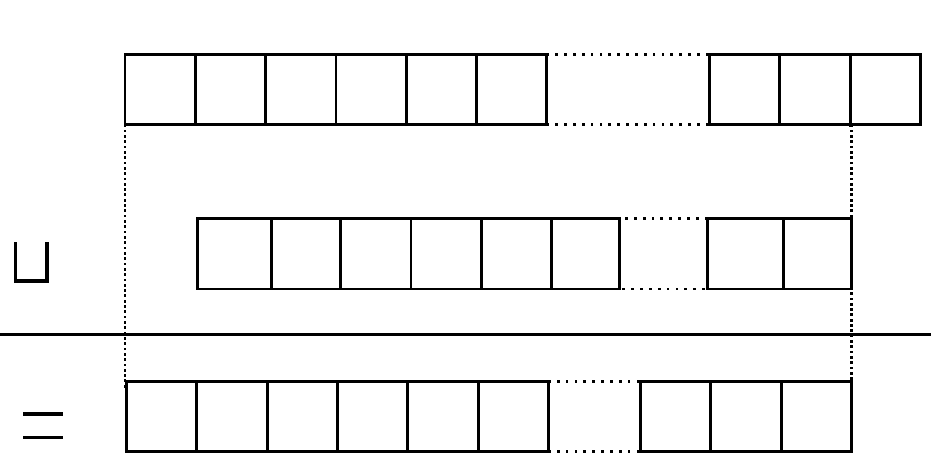
\includegraphics[width=7cm]{cuptype.pdf}
\vspace{0.2cm}
\hrule
    \caption{    \label{figsuptype}The supremum operator $\sqcup$ of  Equation (\ref{eqsuptype}).}
  \end{center}
\end{figure}


The function \texttt{unifyReal} calls in  a mutually recursive way the function \texttt{unify}
on terms. It also refers to type variables correspndig the constructor \texttt{TypeVar}.
The fields of \texttt{TypeVar} are the value itself and a string corrsponding to
the name of the variable. The value may be either \texttt{None} when the type
variable is not constrained or some reference to an expression when a type has been given to the variable
by unification. The function \texttt{solve} performs a partial evaluation of the expressions
occurring in the equations, in order to simplify them, translates them for \texttt{Z3},
calls the SMT solver and then assign the values of the solution to the relevant type
variables. The function \texttt{solveLT} acts just like the function \texttt{solve} but
requires that the precision of the second expression is greater than or equal to the precision of the first
expression instead of a strict equality.
Several cases are distinguished in the function \texttt{unifyReal} of Figure \ref{unireal}:
\begin{itemize}
\item If $\phi_1$ and $\phi_2$ are fully instantiated, i.e.  $s_i,u_i$ and $p_i$, $1\le i\le 2$
are integers then we assign $\phi=\phi_1 \sqcup\phi_2$ to $\phi_1$ and $\phi_2$.
The supremum $\sqcup$ refers to the order $\sqsubseteq$ introduced in  Equation (\ref{eqlttype}).
Formally, we have:
\begin{equation}\label{eqsuptype}
\phi_1\sqcup\phi_2=\big\{ s_1 \uplus s_2,\max(u_1,u_2),p\big\}\ \text{with}\ p=\left\{
\begin{array}{l}
\min(p_1,u_1-u_2+p_2)\ \text{if}\ u_1\ge u_2\enspace ,\\
\min(p_2,u_2-u_1+p_1)\ \text{otherwise}\enspace .
\end{array}\right.
\end{equation}
In Equation (\ref{eqsuptype}), $\uplus$ computes the supremum of to values of \textsf{Sign}.
Figure \ref{figsuptype} illustrates the effect of the operator $\sqcup$.
\item If $\phi_1$ is fully instantiated and $\phi_2$ is made of three type variables then $\phi_1$
is assigned to $\phi_2$.
\item If $\phi_1$ is fully instantiated and $\phi_2$ is neither fully instantiated or a triple
of type variables then $\phi-2$ is made of three integer expressions containing type variables,
$\phi_2=\{e_0,e_1,e_2\}$. We have to solve the system 
\begin{equation}
(S)\ : \ \left\{
\begin{array}{l}
s_1 = e_0\\
u_1 = e_1\\
p_1 = e_2
\end{array}\right.\enspace .
\end{equation}
We call the SMT solver \texttt{Z3} to solve this system of equation. Recall that $e_0$, $e_1$ and
$e_2$ come from the types of primitives introduced in Figure \ref{figtypprim}. These expressions
are linear and are easy to solve for an SMT solver.
\item If both $\phi_1$ and $\phi_2$ are made of type variables then we identify them in a pairwise
manner.
\item If both $\phi_1$ and $\phi_2$ are integer expressions then 
$\phi_1=\{e_0,e_1,e_2\}$ and $\phi_2=\{e'_0,e'_1,e'_2\}$. We have to solve the system 
\begin{equation}
(S)\ : \ \left\{
\begin{array}{l}
e_0 = e'_0\\
e_1 = e'_1\\
e_2 = e'_2
\end{array}\right.\enspace .
\end{equation}
Again, we call \texttt{Z3} to solve this system of linear equations.
\item The other cases are symmetric to the ones detailled formerly, they are treated similarly.
\end{itemize}


\begin{figure}[t]
\begin{center}\tt\scriptsize
\hrule
\vspace{0.2cm}
\begin{tabular}{lll}
\begin{lstlisting}[mathescape]
($\mathbf{assert}$ (= 2 
  ($\mathbf{ite}$ ($\mathbf{and}$ (= a 0) (= 1 0)) 0 
   ($\mathbf{ite}$ ($\mathbf{and}$ (= a 1) (= 1 1)) 1 
    ($\mathbf{ite}$ ($\mathbf{and}$ (= a -1) (= 1 -1)) -1 
     ($\mathbf{ite}$ ($\mathbf{and}$ (= a 1) (= 1 0)) 1 
      ($\mathbf{ite}$ ($\mathbf{and}$ (= a 0) (= 1 1)) 1
       ($\mathbf{ite}$ ($\mathbf{and}$ (= a -1) (= 1 0)) -1 
        ($\mathbf{ite}$ ($\mathbf{and}$ (= a 0) (= 1 -1)) -1 
         ($\mathbf{ite}$ ($\mathbf{and}$ (= a 1) (= 1 -1))
  ($\mathbf{ite}$ (> (+ ($\mathbf{ite}$ (>= b -7) b -7) 
   ($\mathbf{ite}$ ($\mathbf{and}$ (= a 0) (= 1 0)) 0 
    ($\mathbf{ite}$ ($\mathbf{and}$ (= a 1) (= 1 -1)) -1 
     ($\mathbf{ite}$ ($\mathbf{and}$ (= a -1) (= 1 1)) -1 
      ($\mathbf{ite}$ ($\mathbf{and}$ (= a -1) (= 1 -1)) 1 
       ($\mathbf{ite}$ ($\mathbf{and}$ (= a 1) (= 1 1)) 1 
        ($\mathbf{ite}$ ($\mathbf{and}$ (= a 1) (= 1 0)) 0 
         ($\mathbf{ite}$ ($\mathbf{and}$ (= a 0) (= 1 1)) 0
          ($\mathbf{ite}$ ($\mathbf{and}$ (= a -1) (= 1 0)) 0 
  ($\mathbf{ite}$ ($\mathbf{and}$ (= a 0) (= 1 -1)) 0
       2)))))))))) -7) 1 
   ($\mathbf{ite}$ (< (+ ($\mathbf{ite}$ (>= b -7) b -7) 
    ($\mathbf{ite}$ ($\mathbf{and}$ (= a 0) (= 1 0)) 0 
     ($\mathbf{ite}$ ($\mathbf{and}$ (= a 1) (= 1 -1)) -1 
      ($\mathbf{ite}$ ($\mathbf{and}$ (= a -1) (= 1 1)) -1 
       ($\mathbf{ite}$ ($\mathbf{and}$ (= a -1) (= 1 -1)) 1 
        ($\mathbf{ite}$ ($\mathbf{and}$ (= a 1) (= 1 1)) 1 
         ($\mathbf{ite}$ ($\mathbf{and}$ (= a 1) (= 1 0)) 0 
          ($\mathbf{ite}$ ($\mathbf{and}$ (= a 0) (= 1 1)) 0
  ($\mathbf{ite}$ ($\mathbf{and}$ (= a -1) (= 1 0)) 0 
    ($\mathbf{ite}$ ($\mathbf{and}$ (= a 0) (= 1 -1)) 0
         2)))))))))) -7) -1 2)) 
\end{lstlisting}
& &
\begin{lstlisting}[mathescape]
($\mathbf{ite}$ ($\mathbf{and}$ (= a -1) (= 1 1)) 
 ($\mathbf{ite}$ (< (+ ($\mathbf{ite}$ (>= b -7) b -7) 
  ($\mathbf{ite}$ ($\mathbf{and}$ (= a 0) (= 1 0)) 0 
   ($\mathbf{ite}$ ($\mathbf{and}$ (= a 1) (= 1 -1)) -1 
    ($\mathbf{ite}$ ($\mathbf{and}$ (= a -1) (= 1 1)) -1 
     ($\mathbf{ite}$ ($\mathbf{and}$ (= a -1) (= 1 -1)) 1 
      ($\mathbf{ite}$ ($\mathbf{and}$ (= a 1) (= 1 1)) 1 
       ($\mathbf{ite}$ ($\mathbf{and}$ (= a 1) (= 1 0)) 0 
        ($\mathbf{ite}$ ($\mathbf{and}$ (= a 0) (= 1 1)) 0
         ($\mathbf{ite}$ ($\mathbf{and}$ (= a -1) (= 1 0)) 0 
          ($\mathbf{ite}$ ($\mathbf{and}$ (= a 0) (= 1 -1)) 0
            2)))))))))) -7) 1 
 ($\mathbf{ite}$ (> (+ ($\mathbf{ite}$ (>= b -7) b -7) 
  ($\mathbf{ite}$ ($\mathbf{and}$ (= a 0) (= 1 0)) 0 
   ($\mathbf{ite}$ ($\mathbf{and}$ (= a 1) (= 1 -1)) -1 
    ($\mathbf{ite}$ ($\mathbf{and}$ (= a -1) (= 1 1)) -1 
     ($\mathbf{ite}$ ($\mathbf{and}$ (= a -1) (= 1 -1)) 1 
      ($\mathbf{ite}$ ($\mathbf{and}$ (= a 1) (= 1 1)) 1 
       ($\mathbf{ite}$ ($\mathbf{and}$ (= a 1) (= 1 0)) 0 
        ($\mathbf{ite}$ ($\mathbf{and}$ (= a 0) (= 1 1)) 0
         ($\mathbf{ite}$ ($\mathbf{and}$ (= a -1) (= 1 0)) 0 
          ($\mathbf{ite}$ ($\mathbf{and}$ (= a 0) (= 1 -1)) 0
            2)))))))))) -7) -1 2))
     2)))))))))))
\end{lstlisting}
\end{tabular}
\vspace{0.2cm}
\hrule
\end{center}
\caption{\label{figz3}\texttt{Z3} encoding of the first equality of Equation (\ref{exsmteq}).}
\end{figure}

For example, the equations sent to the SMT solver for 
the call \texttt{newton 9.0 0.0 g gprime ;;} to 
the  \texttt{newton} function
of Section \ref{over} are given in Equation (\ref{exsmteq}).

\begin{equation}\label{exsmteq}
(S)\ :\ \left\{
\begin{array}{l}

\mathcal{S}_+( \mathtt{'a}, \max( \mathtt{'b}, -7) + \mathcal{S}_\times( \mathtt{'a}, 1), 1, -7)=2\\
\ \\
(\max (\mathtt{'b}, -7) + \mathcal{S}_\times (\mathcal{S}_+ (\mathtt{'a}, \mathtt{'b}, 1, -7), 1)=10\\
\ \\
\max (\max( \mathtt{'b}, -7) + \mathcal{S}_\times (\mathcal{S}_+ (\mathtt{'a}, \mathtt{'b}, 1, -7), 1), -7) \\
+ 
\mathcal{S}_\times (\mathcal{S}_+ (\mathtt{'a}, \max (\mathtt{'b}, -7) + \mathcal{S}_\times( \mathtt{'a}, 1), 1, -7), 1)\\ 
- \max (\max( \mathtt{'b}, -7) + \mathcal{S}_\times (\mathcal{S}_+(\mathtt{'a}, \mathtt{'b}, 1, -7), 1) - \mathtt{'c}, -60)\\ 
- \iota (\max (\mathtt{'b}, -7) + \mathcal{S}_\times (\mathcal{S}_+( \mathtt{'a}, \mathtt{'b}, 1, -7) ,1) - \mathtt{'c} ,-60)
\le 21
\end{array}\right.
\end{equation}
These equations are encoded in \texttt{Z3} by expanding the operators $\max$, $\mathcal{S}_+$,
$\mathcal{S}_\times$, and $\iota$ following the definitions of Figure \ref{figtypprim}.
For example, the \texttt{Z3} encoding of the first equality of
Equation (\ref{exsmteq}) is displayed in Figure \ref{figz3}. Globally, the encoding of the three
equations of Equation (\ref{exsmteq}) is a $1007$ lines long \texttt{Z3} file.
\texttt{Z3} solves these equations in $0.215$ seconds (average measured time on $5$ executions).
